\documentclass[10.5pt]{report}
\usepackage[utf8]{inputenc}
\usepackage[graphicx]{realboxes}
\usepackage{hyperref}
\usepackage{blindtext}
\usepackage{enumitem}
\usepackage{scrextend}
\usepackage{subcaption}
\usepackage[margin=1in]{geometry}
\usepackage[english]{babel}
\usepackage{adjustbox}
\usepackage{array}
\usepackage[UKenglish]{isodate}

\usepackage{tikz}
\usepackage{mathtools}
\usepackage{relsize}
\usetikzlibrary{plotmarks,arrows,positioning,shapes,calc}

\usepackage{lineno}
\linenumbers
\modulolinenumbers[5]

\renewcommand{\baselinestretch}{1.5}
\linespread{1.8}
\graphicspath{ {images/} }

\begin{document}

\title{
{\Huge Automatic and Interpretable Classification of Melanoma}
\vspace{1cm}\\
{Transfer Report}
\vspace{1cm}\\
{University of South Wales}
\vspace{1cm}\\
{
\includegraphics[scale=0.4]{USW-logo.jpg}}
}

\author{Elliot Naylor}
\date{\today}

\tikzstyle{box} = [rectangle, minimum width=2.4cm, minimum height=0.8cm,text centered, draw=black, node distance=2.5cm, fill=white!30, rounded corners=3]

\tikzstyle{small} = [rectangle, minimum width=0.5cm, minimum height=0.5cm,text centered, draw=black, node distance=4cm, fill=white!30]

\tikzstyle{img} = [rectangle, minimum width=1cm, minimum height=1cm, node distance=2cm, fill=white!30]

\maketitle
\tableofcontents
\listoffigures
\listoftables

\newpage

\chapter*{Abstract}

Melanoma is a dangerous skin cancer where early detection is essential for successful treatment. Computer-Aided diagnostic procedures for the automatic detection of melanoma could benefit patient survival rates. Unfortunately, while many current machine learning techniques produce outstanding accuracy they produce poor explanations, making it difficult for a general practitioner (GP) to utilise in a clinical environment. Nevertheless, doctors frequently utilise diagnostic procedures to diagnose melanoma, the most popular ABCD rules (asymmetry, border, colour, and dermoscopic structures). This work discusses feature extraction algorithms for automating ABCD rules to produce melanoma detection algorithms suitable for GPs. Implemented feature detection algorithms are bi-fold asymmetry measurements and fractal box-counting border detection. Skin lesion segmentation uses LBPC instead of SegNet to detect border irregularity using fractal box-counting. LBPC improved border detection and might improve other techniques for measuring the ABCD rules. Furthermore, bi-fold colour asymmetry was improved using superpixels to create a flexible border to avoid features. Future work will use the extracted features to train Support Vector Machine (SVM) and combine them with Bayesian Fusion.

\chapter{Introduction}

Skin cancer is considered amongst the most severe public health concerns, with mortality rates of 2,353 per 100,000 within the United Kingdom (UK) in 2018 \cite{UK2019}. Skin cancers can be categorised between melanoma and non-melanoma, whereas melanoma is the most dangerous because it is unpredictable. When left untreated and after growing sufficiently, it can spread to other regions of the body (known as metastatic melanoma), which once progressed is challenging to treat effectively with a 10\% survival over ten years in the US \cite{bhatia2009}. Furthermore, it is beneficial to catch melanoma early because it is the most easily treatable form of cancer, with 86\% of cases being preventable \cite{UK2019}. However, melanoma can remain dormant from anywhere between 6-months to 10-years before maturing and becoming a danger to the patient \cite{UK2019}. Another danger of melanoma is its similarity to non-melanoma skin cancers, such as the mimic called seborrhoeic keratosis (SK), which frequently leads to misdiagnoses \cite{Izikson2002}. There are features unique to SK called fissures, ridges, and hairpin vessels \cite{Minagawa2017}. Problematically these features require trained specialists to recognise them needing more than ten years of experience to have an accuracy of 86\% compared to 62\% or 56\% (3-5 years of experience) \cite{Morton1998}. However, because of the cost of training new doctors, there are limited available. Dermatologists primarily treat skin conditions (biopsies) and confirm diagnoses submitted by GP. General practitioners (GP) are the first to diagnose skin conditions and sometimes have limited experience diagnosing skin conditions (especially dermatological features). This project aims to improve the accuracy of GP observations by providing tools for the automatic classification of skin lesions. An automatic system should be cost-effective and advantageous to doctors.

%Diagnostic procedures
Diagnostic procedures are instructions developed by doctors to simplify diagnosing conditions. Various methods have been developed to diagnose skin lesions and have greatly improved GP accuracy within clinical environments \cite{Nachbar, unlu2014}. Considering melanoma is the most dangerous skin condition, most procedures were developed specifically for early detection. Some include ABCD rules, 2-point checklist, 7-point checklist, and CASH. The most preferred of these techniques is ABCD rules and CASH because they have a higher sensitivity \cite{unlu2014} and ABCD rules is generally the most preferred because it is easy to learn and is rapidly calculated \cite{Nachbar}. There are several variations of ABCD rules, but, is originally measured using asymmetry, border, colour, and diameter. Diameter is sometimes replaced with dermatological structures because many features (i.e. blue-black signs, pigment networks, pseudopods, streaks, or milia-like cysts \cite{Stricklin2011}) improve the classification accuracy between melanoma and the mimic seborrheic keratosis \cite{Cognetta1994}. Furthermore, automatically measuring diameter is often difficult because it is dependant on the photo apparatus and the distance from the skin lesion, which is rarely consistent between research. Table \ref{TDS} describes each rule in more detail, including a scoring system called total dermoscopy score (TDS), where each rule is assigned a score and combined to reach a result of either malignant, suspicious or benign. The criteria is: [(Asymmetry $\times$ 1.3) + (Border $\times$ 0.1) + (Colour $\times$ 0.5) + (Dermoscopic structure $\times$ 0.5)]. Each rule is calculated using the following descriptions in Table \ref{TDS} and multiplied by their weight and then added together to reach a final score where [$<$ 4.76 = benign, $>$ 4.76 or $<$ 5.45 = suspicious, $>$ 5.45 = melanoma]. The disadvantage is the subjectivity of GPs observations relating to their experience. So, it would be beneficial to automate the techniques using algorithms to standardise results and improve GP accuracy.

\begin{table}
\small
\begin{tabular}{|p{2.5cm}|p{10cm}|c|c|}
	\hline
	Criteria & Methodology & Score & Weight \\
	\hline
	Asymmetry & Measuring asymmetry involves firstly finding the centroid and splitting it twice with a 90 degree axis. Each side is subtracted with its opposite half to measure the asymmetry of shape, colour, and dermoscopic structures. If both sides are asymmetrical then the score is 2, one side asymmetrical is a score of 1, otherwise the score is 0. & 0 - 2 & $\times$ 1.3 
	\\
	\hline
	Border & border is found by finding the centroid and drawing lines through it with a 45-degree angle, splitting the skin lesion into eight segments. Border segments might be irregular with convexity, sharp corners, or edges. Irregular segments are incremented by 1, reaching 8 for each segment.  & 0 - 8 & $\times$ 1.3 
	\\
	\hline
	Colour & The area of the skin lesion hs up to 6 colours (white, red, light brown, dark brown, blue-grey, black). The score is increased by 1 for each visible colour, reaching a total of 6. & 1 - 6 & $\times$ 0.5 
	\\
	\hline
	Dermoscopic Structures & Dermoscopic structures are measured by finding structureless areas, pigment networks, atypical networks, dots, and globules. Each visible structure adds a score of 1, reaching a total of 5. & 1 - 5 & $\times$ 0.5 
	\\
	\hline	
\end{tabular}
\caption{Total dermoscopy score (TDS) is a scoring system used with ABCD rules to support clinicians when diagnosing melanoma \cite{Cognetta1994}. Each rule is multiplied by weights and the sum of the combined values is the final score, altogether: [(Asymmetry $\times$ 1.3) $+$ (Border $\times$ 0.1) $+$ (Colour $\times$ 0.5) $+$ (Dermoscopic structure $\times$ 0.5)].}
\end{table} \label{TDS}

%What type of CAD framework
Computer-aided diagnostic (CAD) frameworks are a collection of algorithms designed to guide decision making processes within clinical environments \cite{Dick2019}. A paper written by Andre Estava demonstrates a Deep convolutional neural network (DCNN) that has comparable accuracy to that of dermatologists, trained using 129,450 clinical images consisting of 2,032 different diseases \cite{Andre2017}. DCNN generates a collection of artificial neurons organised into layers, where each neuron receives an input from a previous layer to perform a computation. The collection of layers is a network, which (once trained) ultimately measures the relationship between input parameters based on provided data. It is important to note that the accuracy is proportionate to the number of images and data quality for training that network. Unfortunately, these image samples are frequently private and unavailable to many institutions. Without adequate image data to test the capabilities of machine learning models, there is no method for measuring these biases and is therefore unsafe to use within clinical environments. Secondly, these approaches will often produce a parallel diagnosis, not explaining the results. There are many valuable techniques, but even the best techniques are inadequate for doctors without catering to interpretability. Other techniques are interpretable by considering diagnostic procedures, such as ABCD rules, many of which are described by Ali \cite{Ali2020}. Techniques based on diagnostic procedures can be more easily tested for biases and provide further insight to GPs with the means to learn from and understand the results. Techniques include support vector machine (SVM), a supervised machine learning that uses regression analysis to categorise labelled data into two or more groups. The advantage means less data for training is required, and the model is interpretable.

Explainable AI (XAI) techniques have recently gained attention because the European general data protection regulation (GDPR and ISO/IEC 27001) stated that these approaches, commonly referred to as ``black box'' approaches, are challenging to utilise in medical environments. Since then, There has been significant progress in making neural network architectures more interpretable. A wide range of techniques \cite{Fuji2019,  Selvaraju2016, Ribeiro2016} have since been developed, demonstrating that it is possible to make neural network techniques interpretable. However, the problem is instead the current scepticism on whether these techniques are trustworthy \cite{Tjoa2019, Samek2019a}, and they can produce realistic but incorrect results \cite{Ghorbani2019}. Some other interpretable techniques do not utilise neural networks. For example, Javier López-Labraca et al. \cite{Lopez-Labraca2018} described an interpretable technique using multiple SVM models with colour and three dermoscopic structures (i.e., pigment networks, globules, and streaks). Bayesian fusion combines each model to calculate a diagnosis. Bayesian probability is a type of probability theory that uses probability distribution to estimate the values of unobserved variables. Bayesian fusion has a comparable accuracy to neural network techniques \cite{Takruri2017}. Therefore, overall results should be partially interpretable for use within clinical environments.

% Visualisation
Doctors will often only have access to a patient for a short time before moving to another. CAD frameworks are beneficial because they speed up the process, can improve accuracy \cite{Dick2019}, and ensure the gathering of relevant data (ABCD rules). Furthermore, it could take days for a second opinion from another doctor, where an automatic system immediately provides it. Automated systems should also provide adequate explanations that can be understood quickly and easily by doctors. One method is to provide visual explanations. Many authors \cite{Zaqout2016, Kasmi2016a, Ali2020a} describe different ways to measure ABCD rules, including the asymmetry of skin lesions using bi-fold. Automated versions of the procedure use the centroid and moments of inertia to fold the skin lesion horizontally and vertically along the centroid. The overhung area on both axes is subtracted from the final score to measure asymmetrical or symmetrical. This technique produces an adequate visualisation that can provide GPs with an interpretable result. There is a range of other examples for ABCD rules, including border \cite{Kasmi2016a, Zaqout2016, Ali2020b}, colour \cite{She2007, Tenenhaus2010, Kasmi2016a}, and dermoscopic structures \cite{Lopez-Labraca2018} that use a range of interpretable algorithms that produce interpretable results.

%Conclusion
Overall, many advanced machine learning techniques using neural networks lack the interpretability required within clinical environments. Furthermore, public datasets lack rarer skin conditions, making finding biases challenging. Automating the ABCD rules can solve this by using a technique that GPs are familiar with, by using statistical models to extract relevant features (relating to the ABCD rules). This is followed by summarising rules using Bayesian fusion and calculating the significance of individual features.

\section{Aim}
\begin{itemize}
	\item Develop an interpretable CAD framework based on the ABCD rules to diagnose skin lesions automatically. The goal is to utilise statistical models to extract each ABCD rule (asymmetry, border, colour, and Dermoscopic structure). Each rule will be trained using individual SVM models and are combined using Bayesian Fusion.
\end{itemize}

\section{Objectives}
\begin{itemize}

	\item Develop and validate skin lesion segmentation and border cut-off approach for improved irregularity detection of ABCD rules using SegNet and LBPC.
	\item Develop and validate melanoma classification based on the diagnostic procedure ABCD rules (asymmetry, border, colour, and dermoscopic structures) for improved interpretability to doctors using various statistical techniques and SVM models.
	\item Develop and validate combining ABCD rules for the probabilistic analysis of the most dependent features using Bayesian fusion. This could include meta-data for gender, age, touch, feeling, and location on the body.

\end{itemize}

\section{Contributions to knowledge}
 
\begin{enumerate}

\item \textbf{Developing and validating a novel skin lesion segmentation approach for accurate border cut-off segmentation to improve border irregularity analysis using SegNet and LBPC.}

SegNet is highly accurate at finding the area for the segmentation of skin lesions but is inaccurate for measuring border irregularities because the border cut-off between skin and skin lesion is insufficient. Border irregularity detection necessitates an accurate cut-off for more reliable results, which SegNet does not provide. LBPC solves this problem by exaggerating the cut-off and improving the accuracy of border irregularity detection. However, the disadvantage of LBPC is its inaccuracy when finding the skin lesion area. By combining SegNet and LBPC, detecting the skin lesion area using SegNet, followed by adjusting the border with LBPC; this should retain the accuracy of SegNet while improving the border cut-off accuracy. Experimental testing utilising the PH$^2$ dataset containing expert segmentation data will determine the benefits of segmentation.

\item \textbf{Developing and validating a novel asymmetry analysis approach for improved irregular asymmetry detection in skin lesions using moment-based texture analysis for improved bi-fold analysis and superpixels for improved asymmetry colour comparisons.}

The disadvantage of asymmetry measuring techniques for skin lesions is rotational moments for creating bi-folds. Current bi-folds solely consider the silhouette of the skin lesion, with no consideration towards colour or texture. Furthermore, recent techniques have measured asymmetrical irregularities based on colour and texture. Producing a bi-fold based on the shape, colour, and texture using moment-based texture analysis should improve the accuracy of asymmetry detection. In addition, utilising superpixels to measure colour asymmetry to avoid merging important features improves accuracy. Both techniques will be validated using the PH$^2$ asymmetrical score.  

\item \textbf{Developing and validating a novel interpretable melanoma classifier for improved interpretability of ABCD rules (asymmetry, border, colour, and dermoscopic structures) using feature extraction, support vector machines (SVM), and Bayesian fusion.}

The disadvantage of many neural network-oriented techniques is their lack of adequate interpretability, making them challenging to utilise in clinical environments. However, ABCD rules (asymmetry, border, colour, and dermoscopic structures) are a diagnostic procedure that most doctors are familiar with; therefore, developing a system automating this procedure is beneficial. Feature extraction techniques aim to separate the data essential for each ABCD rule and train an SVM model from the extracted features. For example, bi-folds measure asymmetry, which can be modified to train an SVM model. Repeating this for border, colour, and dermoscopic structures ensures that each rule is independent. Finally, combining the Bayesian fusion results measures the probabilistic significance between ABCD rules and combines them into benign or malignant. Techniques will be validated using the PH$^2$ dataset for testing ABCD rules and ISIC 2018 datasets for diagnosis.

\item \textbf{Developing and validating a novel interpretable melanoma classifier with meta-data including age, gender, feeling, and location on the body to improve classification accuracy between melanoma and seborrhoeic keratosis (SK) using Bayesian probability for a modifiable probabilistic analysis.}

Seborrhoeic keratosis (SK) is a melanoma mimic because it sometimes shares clinical features with melanoma. Moreover, differentiating between the two with entirely image data can lead to inaccuracies. Including meta-data age, gender, feeling, and location on the body should improve accuracy because SK appears more frequently on the head or back of old male patients. Bayesian probability networks are considered highly modifiable and can generate results with incomplete input, meaning meta-data is only inputted when necessary, benefiting doctors and improving the diagnosis. The associated organisation has a vast amount of valuable meta-data alongside image data of skin lesions; a private dataset will be created from these results and used to validate results.


\end{enumerate}

\chapter{Literature Review}

\section{Introduction}
This chapter reviews statistical and machine learning algorithms for the automatic classification of ABCD rules and discusses techniques beneficial to clinical environments.

\section{Discussion}
When doctors diagnose conditions using CAD, they should rationalise and build an explanation to prove their diagnosis, building criteria that other doctors understand. Currently, many techniques \cite{Andre2017} called ``black box'' approaches produce what is called a parallel diagnosis that lacks an explanation. These are insufficient for use within some clinical environments for this reason. Instead, it would be beneficial for doctors to follow procedures they are familiar with, such as diagnostic procedures, ABCD rules. The reviewed techniques aim to automate the ABCD rules using various statistical and machine learning techniques. Many are interpretable and suitable for clinical environments.

Hybrid machine learning techniques are recently gaining traction, an example by Ali combines results from both Gaussian naive Bayes (GNB) and a CNN \cite{Ali2020b} for border irregularity detection. The CNN ensures the high accuracy classification by finding the relationship between each component, and the GNB is interpretable. Results are combined using an ensemble approach, making a prediction probability. Such techniques are promising for use within clinical environments.

There is a lack of literature describing adequate visual representations for doctors, and it is understandable as there is still little evidence proving that CAD systems improve doctors decision making-processes \cite{FerrantediRuffano2018}. It would be beneficial to create literature describing a catalogue of different visualisations that benefit doctors. Putting all this information together, alongside a questionnaire, might provide further insight into the visualisations that might be most useful to doctors.

\subsection{Datasets}
One fundamental problem is the overutilisation of private or privately annotated datasets, making a direct comparison of algorithms difficult; hence, this review has no direct comparisons. Some are between benign and malignant \cite{Meskini2018, Kasmi2016a, Ali2020b, Ali2020a} while others utilise private or never mention any datasets \cite{Kasmi2016a, She2007, Tenenhaus2010, Ramezani2014, Zaqout2016}. None compare their rules, likely because of subjectivity depending on the dermatologists that labelled them. More datasets should be public to assess individual rules and reach objective measurements. Until then, results conform with malignant, suspicious, or benign.

\section{Previous Works on Automating ABCD Rules}
Many CAD frameworks follow a methodology for the classification of skin lesions. These are listed below:

\begin{enumerate}
	
	\item Segmentation – Image segmentation is the process of partitioning an image into multiple segments for more accessible analysis. These areas can be separated manually by a dermatologist (known as the ground-truth) or separated automatically using statistical or machine learning algorithms.
	
	\item Feature Extraction - Gathering features through filtering, morphology and other statistical approaches. ABCD rules include asymmetry, border, colour, and dermoscopic structures.

	\item Combination - Combining the extracted features before using Principal Component Analysis (PCA) or after classification using Bayesian Fusion. Others combine the results using the Total Dermoscopy Score (TDS).
	
	\item Classification – Measuring the results from the features and components through classification. Containing the final diagnosis of the type of skin lesion (Naveus, SK, or Melanoma)

\end{enumerate}

\subsection{Segmentation}
Yading Yuan and Yeh Chi Lo describe a fully convolutional network (FCN) with an accuracy of 91.7\% with the PH$^2$ dataset \cite{Yuan2017a}. FCN is a variation of a CNN using 1x1 convolutions instead of dense layers. Essentially, an FCN forms a more complex function (generating a more complex neural network), whereas the CNN forms a less complex function, likely to degrade essential features. Therefore, more data is needed to train an FCN effectively than a CNN. After the convolution layers, transposed convolution layers (or deconvolution) and other layers (un-pooling) up-sample the input feature map to the size of the input image. Then, the network, trained from ground truth (human-generated segmentation mask) and the original images, can automatically generate segmentation masks based on textures and colours of the skin lesion provided. There are dozens of examples of this, such as SegNet \cite{Badrinarayanan2017}, which is another transposed CNN not designed initially for skin lesions but is effective at segmenting skin lesions.

E. Meskini et al. proposed using Otsu binarisation - a threshold technique that is effective at locating the border of a skin lesion after segmenting using Segnet \cite{Meskini2018}. Researchers proposed that when analysing the skin lesion border using ABCD rules, the original SegNet methods were ineffective because the ground-truth is subjective - ineffective at finding the border cut-off between the skin lesion and skin. While SegNet has a 91.7\% with the PH$^2$ dataset, the data is not effective at finding the precise border cut-off required for accurate border classification using ABCD rules. Therefore, researchers proposed the Otsu threshold to find the skin lesion border after segmenting using SegNet. Fan proposes another technique that uses a saliency-based segmentation approach to capture the area, followed by an Otsu threshold \cite{Fan2017} to find the border cut-off from the skin lesion with a precision of 96.78\% validated using the PH$^2$ dataset.

Pedro M.M. Pereira et al. proposed local binary pattern clustering (LBPC) to exaggerate the border, producing accurate results when classifying ABCD rules than ground-truth borders in the PH$^2$ dataset \cite{Pereira2020}. Local binary patterns (LBP) are texture descriptors calculated by comparing the centre pixel (of each pixel in the grey scaled image) with the eight neighbouring pixels as 'i', and converting it to a binary using the equation:  [$if centroid > neighbour_i =  0, otherwise = 1$]. These eight neighbouring values produce a binary of 01101100 (decimal of 108) and change the centroid to 108. Next, the described process repeats on each other pixel in the image. Finally, the newly filtered image subtracted from the original grey scaled image creates a segmentation mask with an accurate border cut-off. Finally, Pereira describes classification methods using SVM or FNN presenting the extracted border with an accuracy of 79\% and 77\% (respectively) with the MED-NODE dataset.

\subsection{Handcrafted Features}
Handcrafted features are the extraction of particular features using statistical algorithms—the benefit of separating data into components is a more accessible breakdown, improving explainability. In addition, this might instantiate trust for use within a clinical environment and prove more helpful to doctors.

\subsubsection{Asymmetry}
Asymmetry can be measured using the bi-fold technique, which involves drawing a line down the middle of the skin lesion and comparing the two halves to confirm whether the sides match, on both the horizontal and vertical axes, as shown in \ref{lit-asym}. If the two sides are greatly different, it could be a warning sign of melanoma. Asymmetry can be measured using the shape \cite{Zaqout2016}, colour\cite{Kasmi2016a} and texture \cite{Ali2020a}.

\begin{figure} 
\centering
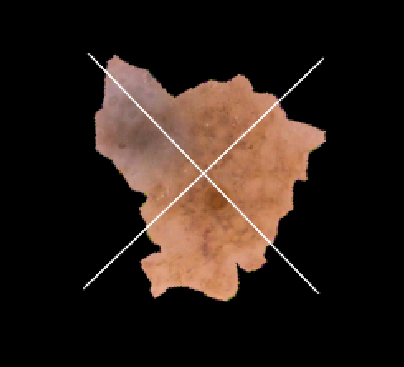
\includegraphics[scale=0.5]{asym1.png}
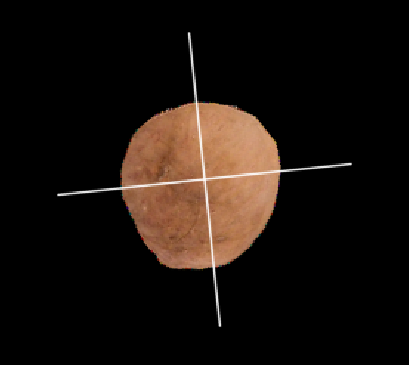
\includegraphics[scale=0.5]{asym2.png}
\caption{Images of two skin lesions from the PH$^2$ dataset showing the asymmetry calculated from moments.}
\end{figure} \label{lit-asym}

Measuring the asymmetrical shape requires a precise border cut-off. Ihab S. Zaqout \cite{Zaqout2016} describes a technique using the centroid and rotation of the skin lesion using moments of inertia. By Folding the skin lesion on both vertical and horizontal axes subtracting the opposite half. Pixels that cannot subtract are summed and compared with a threshold considering the skin lesion asymmetrical if the combined sum is more than the threshold.

Reda Kasmi and Karim Mokrani \cite{Kasmi2016a} describe creating a grid of 20x20 pixels of the skin lesion image and converting it into the LAB colour space. Next, each block's average colour is compared with a perpendicular block (vertical and horizontal axes) using the three-dimensional Euclidean luminance distance, a-axis, and b-axis. If more than half of the colour comparisons are over the threshold, that axis is considered colour asymmetrical. Blocks that have no symmetrical pair are ignored. Finally, luminance calculated separately prevents brightness problems. This technique has an accuracy of 94\% with a private dataset.

Measuring similarities in texture can be achieved by using SIFT based similarity and projection profiles \cite{Ali2020a}. SIFT is scale-invariant and helpful for texture components with varying texture quality. First, the skin lesion is split vertically and horizontally across the centre into four halves, comparing texture components on the symmetrical halves measuring the similarity. Lastly, the projection profile in the x and y directions generate histograms. These results train a decision tree and have an 80\% accuracy of the ISIC 2018 with 204 images privately annotated for ABCD rules and combined.

\subsubsection{Border}
Estimating border irregularities involves splitting the skin lesion into eight equal sections (through the centroid), where each section with tight corners and convexity is considered irregular. Each irregular section of the border adds a score of 1 ranging from 0 to a total of 8, as shown in figure \ref{borders}.

\begin{figure}
\centering
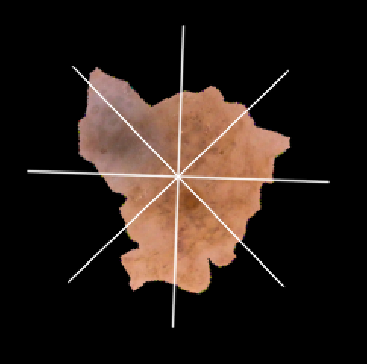
\includegraphics[scale=0.5]{bord1.png}
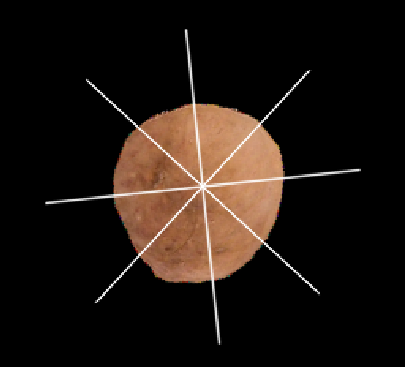
\includegraphics[scale=0.5]{bord2.png}
\caption{Images of two skin lesions split into 8 sections using moments, each is border is measured for irregularity.}
\end{figure} \label{borders}

Border irregularity contours were found by splitting the skin lesion into eight segments around the centre, then calculating a fitting error for each. If the error is larger than the 0.05 (x contour), that area is considered irregular \cite{Kasmi2016a}.

Abder Rahman H. Ali et al. calculate the compactness of each border by first calculating the contour around the area of the lesion containing x and y positions. Next, measure the space between each position to estimate the compactness. The tighter the curves and corners, the more contour positions, revealing irregular borders within a segment, combining all of these scores creates the irregularity index \cite{Zaqout2016}.

Fractal dimensions (FDs) is a statistical index measuring the detail in a pattern changing with the image scale index. One technique called box-counting increases values if there are more corners and edges around the border. The higher the value demonstrates the level of border irregularity. Ali describes using machine learning alongside Zernike moments, and convexity measurements for a high accuracy border irregularity classification \cite{Ali2020b}. However, results are ambiguous because the output is either "irregular" or "regular" border (not relating to the TDS). Thus, conforming to the TDS and splitting the border into eight sections would make it more interpretable and useful o doctors. However, a hybrid GNB and CNN approach are combined to allow interpretability through GNB.

\subsubsection{Colour}
Colour refers to the shades of pigment within the area of a skin lesion, not referring to abnormalities relating to bruises, crust, and grazes. Melanoma usually contains more than two colours compared with benign lesions, singular in colour. Skin lesions can consist of one or many colours: white, red, light brown, dark brown, blue-grey and black.

Finding colour variations has been achieved by calculating the normalised standard deviation of the red, green, and blue components \cite{She2007}. The normalisation process improves the recognition of normal skin pigmentation, which would show pigmentation levels, making comparisons easier between different skin lesions.

Arthur Tenenhaus, et al. utilises joint learning using Kohonen map, and k-means clustering \cite{Tenenhaus2010}. Five random pixels create a 5x5 Kohonen map represented by 25 neurons in a neural network for each skin lesion in the dataset. Colour variations on a 25-dimensional vector find the proportions of pixels projected onto each of the 25 neurons. Next, K-means classifies the skin lesions set by the number of colours found by dermatologists. Only four colours were present in the dataset in this scenario, while seven could be. Eventually, the colour components are represented as a 42-dimensional vector and are passed into a KL-PLS based classifier to detect variations in colour at 66\% using a private dataset.

Reda Kasmi et al. locates the number of colour variations by converting the image into the LAB colour space matching the colour ranges that can be perceived by human eyes \cite{Myridis2014a}, measuring the average colour distribution of the dataset and assigning each colour as a threshold range. Next, the Euclidean distance between each colour threshold is compared with each pixel colour  \cite{Kasmi2016a}, finding the closest matching colour of the six colours. Finally, removing the areas of colour with less than 5\% prevent the classification of dots. This approach uses a colour range of white, light brown and dark brown. However, there is a static threshold value for the other colours, which would be unlikely to cover the ranges of the colours, including red, blue-grey, and black.

\subsubsection{Dermoscopic structures}
Dermoscopic structure refers to structures on the skin lesion, including pigment networks, structureless areas, dots, globules, streaks, white structures, and 22 others (not including sub-types). Variations of pigment networks are more commonly found in melanoma \cite{Anantha04} and are therefore a valuable feature for automatic classification. Similarity other features such as milia-like cysts, a sub-type called milia-like cysts (MLC) called cloudy MLC appears more frequently on melanoma than SK, with a specificity of  99.1\% specificity \cite{Stricklin2011}.

Javier López-Labraca et al. \cite{Lopez-Labraca2018} describes a statistical approach to classifying melanoma using dermoscopic structures through Gabor filtering, support vector machines, and Bayesian fusion. This technique uses a form of soft segmentation to find the area of these dermoscopic features. Firstly the structures are located using Gabor filtering using different values to find fissures and globules. Each structure is then compared with a trained SVM model to check the similarity of the detected features. The results from the model are then combined using Bayesian fusion to reach a result of malignant or benign. Finally, training a CNN model alongside an SVM improves the retractability of dermoscopic structures; compared to a standalone CNN model.

\subsubsection{Combining ABCD Rules}
This section describes combining features from the ABCD rules into a classification between malignant, suspicious or benign after considering all clinical features. Again, meta-data and texture can potentially improve the results.

Maryam Ramezani et al. proposed a method to extract features from ABCD rules storing them in vectors and extracting the texture as a GLCM. First, these 187 features are shrunk to 13 using PCA \cite{Ramezani2014}. Next, the data trains an SVM to classify skin lesions into benign or malignant with an accuracy of 82.2\% on macroscopic images using a private dataset.

Other methods output TDS \cite{Zaqout2016, Zhang2018}, which combines them using: [(Asymmetry x 1.3) + (Border x 0.1) + (Colour x 0.5) + (Diameter x 0.5)]. A statistical model for each ABCD rule outputs a score in the same format. The benefit is interpretability because it follows the diagnostic procedure. The technique achieved an accuracy of 90\% using a private dataset.

\section{Conclusion}
Many techniques utilise ABCD rules to produce an automatic and interpretable diagnosis. Interestingly, many focus on detecting and classifying either asymmetry, border, and colour (ABC) or dermoscopic structures, but neither combine the whole ABCD rules into a single framework. Despite dermoscopic structures providing a means of diagnosing problematic forms of melanoma, including mimics (seborrhoeic keratosis) \cite{Izikson2002}, and non-pigmented melanomas. Thus, it would be valuable to combine both into a single system for possibly higher accuracy.

Despite various valuable features, asymmetry rarely utilises techniques other than statistical models. For example, researchers highly focused on border irregularity and dermoscopic structures, leading to hybrid machine learning models for their assessment. However, asymmetry still utilises statistical approaches to measure and combine the shape, colour, and texture. It would be beneficial to transform this data and process it using an SVM, improving accuracy.

Utilising external data, including feeling, touch, age, and location on the body, are helpful to doctors when diagnosing skin conditions, but are not mentioned in any of the discussed techniques. It would be beneficial to implement this data into the decision-making process.

\chapter{Progress}

\section{Introduction}
This chapter is about automating ABCD rules using statistical models and preparing the data for processing with support vector machines (SVM). This section includes comparisons and small contributions to knowledge.

\section{Model}
The proposed CAD framework described in Figure \ref{model} automates the ABCD rules using statistical algorithms to extract features ($f$) from asymmetry, border, colour, and dermoscopic structures. Each feature has an associated SVM model trained using these extracted features. Next, Bayesian fusion, a probabilistic approach, combines multiple independent classifiers to diagnose melanoma. One benefit of Bayesian fusion is its higher accuracy of classifying skin lesions as compared to a standalone classifier \cite{Takruri2017}.  Javier López-Labraca, et al describe a similar method using dermoscopic structures, and colour \cite{Lopez-Labraca2018}. Other benefits are estimating the relevance of individual classifiers and classifying them with incomplete data, making it an interpretable and robust method. In addition, some feature extraction techniques generate graphics that might be suitable as an explanation for the diagnosis. Finally, the PH$^2$ dataset validates the rules, and once combined into a diagnosis, more extensive datasets, including ISIC 2019, can measure its accuracy.

\begin{figure}
\begin{tikzpicture}[]

	%Image Acqusition
	\node (inp) [img] at (0, 3) {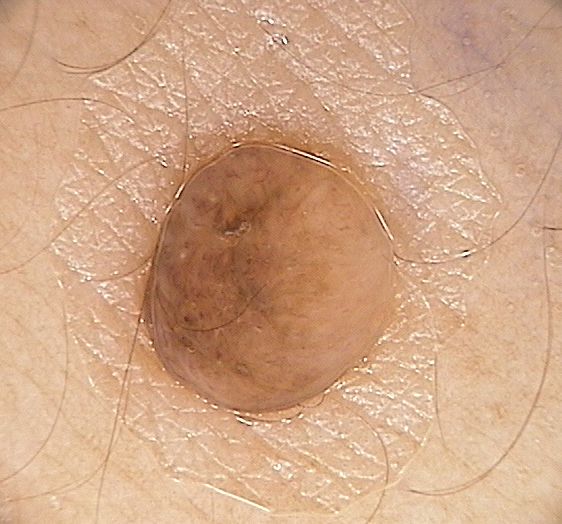
\includegraphics[scale=0.12]{lesion.png}};
	
	%Pre-processing
	\node (aug) [box, minimum height=1cm, node distance=3.6cm, right of=inp] {Augmentation};
	\node (seg) [box, minimum height=1cm, node distance=3.6cm, right of=aug] {Segmentation};
	
\node[draw=white] at ($(aug.north west)+(1.3,0.5)$) {\textbf{Pre-processing}};

\draw[thick, dotted] ($(aug.north west)+(-0.3,0.3)$) rectangle ($(seg.south east)+(0.3, -0.3)$);		

    %Feature extraction
    \node (asy) [box, right of=seg] at (0.0, 0.4) {Asymmetry};
    \node (bor) [box, right of=seg] at (0.0, -0.8) {Border};
    \node (col) [box, right of=seg] at (0.0, -2.0) {Colour};
    
    \node (asy2) [box, minimum width=1cm, right of=asy] {$f_a$};
	\node (bor2) [box, minimum width=1cm, right of=bor] {$f_b$};
    \node (col2) [box, minimum width=1cm, right of=col] {$f_c$};

		\node[draw=white] at ($(asy.north west)+(1.9,0.5)$) {\textbf{Feature Extraction}};    
    
    \draw[thick, dotted] ($(asy.north west)+(-0.3,0.3)$) rectangle ($(col2.south east)+(0.3, -0.3)$);
    
    %Classification
    \node (asy3) [box, right of=asy2] {SVM$_a$};
	\node (bor3) [box, right of=bor2] {SVM$_b$};
    \node (col3) [box, right of=col2] {SVM$_c$};

	\node[draw=white] at ($(asy3.north west)+(1.3,0.5)$) {\textbf{Classification}};    
    
    \node (fus) [box, minimum height=3cm, minimum width=1.7cm, text width=2cm] at (10.56, -0.8) {Bayesian \\ Fusion};
    
    \draw[thick, dotted] ($(asy3.north west)+(-0.3,0.3)$) rectangle ($(fus.south east)+(0.3, -0.3)$);
      
    \node (out) [box, right of=fus, node distance=2.7cm, minimum height=1.9cm, minimum width=1.9cm, text width=2cm] {Benign or \\ Malignant};
    
	\draw[->]
			(aug) edge (seg)
			(asy) edge (asy2)
			(bor) edge (bor2)  
			(col) edge (col2)  
			(asy2) edge (asy3)
			(bor2) edge (bor3)  
			(col2) edge (col3)  
			  
;
	\draw[->] (bor3)
	-|	($(fus.west)+(-0.5, 0)$)
 	|- (fus)
;

	\draw[-] (asy3)
	-|	($(bor3.east)+(0.5, 0)$)
;

	\draw[-] (col3)
	-| ($(fus.west)+(-0.5, 0)$)
;

 	\draw[->] (inp) edge (aug)
 			(asy2) edge (asy3)
			(bor2) edge (bor3)  
			(col2) edge (col3)  
 			(fus) edge (out)
 				(seg) -| ($(seg.east)+(0.7, 0)$)
 					  |- ($(seg.east)+(0, -1.2)$)
 					  -| ($(asy.west)+(-0.8, 0)$)
 					  |- (asy)
;

 	\draw[->] ($(asy.west)+(-0.8, 0)$) 
 		  |- (bor)
;

	\draw[->] ($(asy.west)+(-0.8, -1.2)$) 
 		  |- (col)
; 
    
\end{tikzpicture}
\caption{Proposed CAD framework describing the segmentation, feature extraction  and classification process.} \label{model}
\end{figure}

ABCD rules describe the classification process for each rule and demonstrate the process behind reaching diagnoses. The objective is to visualise important features that GPs might need to support their diagnostic procedure. Hopefully, this will instantiate trust when automating skin lesion identification within clinical environments. Another advantage would be the automatic labelling of skin lesions, making it easier for dermatologists to identify later.

The CAD framework in figure \ref{model} describes a model of pre-processing, feature extraction, and classification stages. After segmentation, statistical algorithms extract features ($f$), representing a different rule. Next, SVM models individually process the extracted features and combine them into a final result between benign and malignant using bayesian fusion.

\section{Skin Lesion Segmentation}
This section discusses segmentation techniques producing statistically significant border cut-off at the perimeter of the skin lesion. An accurate border cut-off is an essential criterion for melanoma detection \cite{Pereira2020, Kaya2016} using ABCD rules. Unfortunately, segmentation continues to be a challenging task because datasets regularly contain an estimated border but sometimes an inaccurate border cut-off.

\subsection{Local Binary Patterns Clustering (LBPC)}
Local Binary Patterns (LBP) is a texture descriptor commonly used for augmenting the image improving classification accuracy \cite{Pereira2020, Kaya2016}. First, equation \ref{eq1} calculates each pixel, where $p$ (equal to 8) is the number of neighbouring pixels compared to the centre of $c$, and radius of $r$ from the centre. Next, shown in equation \ref{eq2} each value is subtracted counter-clockwise with the centre value and compared to function $S$ where each $gp - gc$, if more than or equal to 0, is equal to 1, and less than 0 is equal to 0. Next, add corresponding values equal to 1 of $gp$ together, changing the centre value, ignoring values of 0. Next, applying a Gaussian kernel of 13-pixel iterations and a standard deviation of 3 removes smaller features that interfere with the segmentation. Finally, applying k-means with a value of 2 subtracts the greyscale and segments the skin lesion from the skin.

\begin{equation} \label{eq1}
LBP(gp_x, gp_y) = \mathlarger{\sum}_{p=0}^{P-1}s\big(gp - gc)2^p
\end{equation}

\begin{equation} \label{eq2}
s\big(x) = 
\begin{cases}
1,\:\:x\geq\:0; \\
0,\:$otherwise$.
\end{cases}
\end{equation}

Figure \ref{fractal1} demonstrates the segmentation of two skin lesions, one with an irregular border and another with a regular border. LBPC is applied to both skin lesions, followed by Gaussian blurring and morphology closing to remove dots. The result is an improved border cut-off compared to the ground-truth in the Ph$^2$ dataset with more corners and ledges. This technique will improve accuracy for measuring border irregularity \cite{Pereira2020}.
 
\begin{figure}
\centering
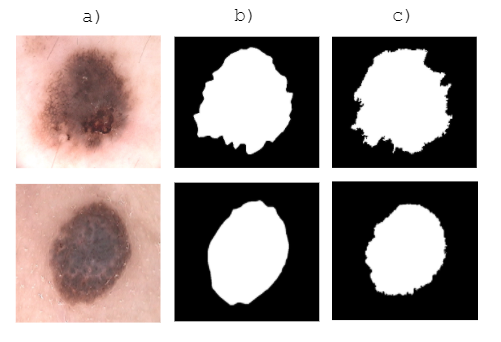
\includegraphics[scale=1.2]{borders.PNG}
\caption{Local Binary Pattern Clustering (LBPC) showing the a) original image, b) ground-truth, and c) LBPC. LBPC successfully exaggerates the border cut-off on the skin lesions with regular and irregular borders} 
\end{figure} \label{fractal1}

Validating LBPC is not expected because the goal is to exaggerate the border to improve the classification process of ABCD rules, which it does successfully \cite{Pereira2020, Kaya2016}. For example, the segmentation might not match dataset segmentations but is still essential to classifying ABCD rules. Furthermore, many datasets lack expert border segmentation, an accurate border cut-off between the skin and skin lesions, so comparisons are not always possible.

\subsection{Semantic Pixel-Wise Segmentation}
Semantic pixel-wise segmentation (SegNet) is a machine learning architecture utilising a deep, fully convolutional neural network (DCNN). This network requires training from ground-truth and pre-segmented images for automatic segmentation. SegNet consists of encoding layers, decoding layers, and a pixel-wise classification layer. The encoder layers consist of 3x3 convolutions (including batch normalisation and ReLU), pre-trained filters for classifying features. After some convolutions, the data is down-sampled using a 2x2 pooling layer. Next, decoding layers consist of up-sampling, followed by 3x3 convolutions. Finally, the pixel-wise classification uses a softmax layer to represent each pixel between 0 and 1 based on the previous layers, generating a segmentation mask.

\begin{figure}[hb]
\centering
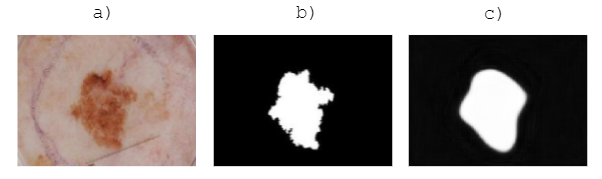
\includegraphics[scale=1.2]{border-seg.png}
\caption{Demonstrating the Semantic Pixel-Wise Segmentation (SegNet) results showing the a) original image, b) expert ground-truth and c) SegNet results.} \label{SegNet}
\end{figure}

Results in figure \ref{SegNet} are generated from the architecture using the ISIC 2018 dataset split into 80\% training and 20\% validation images. The accuracy of locating the lesions is 85\%. However, figure \ref{SegNet} represents the border cut-off between skin and skin lesion is accurate to the dataset but inadequate for using the ABCD rules. Finding the border cut-off is vital for measuring ABCD rules \cite{Pereira2020}.

\subsection{Otsu Thresholding}
Otsu threshold is a versatile automatic image thresholding technique meant to separate each pixel between two classes of foreground or background. One of the benefits of this method is that it does not require any training data. The equation \ref{otsu} (within-class variance) describes splitting weights of $w_0(t),w_1(t)$, which are the probabilities divided by the threshold $t$, between 0 to 255. Furthermore, $\sigma_1^2$ and $\sigma_0^2$ are variances of these two classes. The class probability $w$ is computed from the histogram in figure \ref{otsu2}, which is an intensity histogram describing the colour distribution in an image. Measuring the values above and below the generated thresholds splits the image into two classes.

\begin{equation} \label{otsu}
\sigma_w^2(t) = w_0(t)\sigma_1^2(t) + w_1(t)\sigma_2^2(t)
\end{equation}

The histogram is split into two segments with the threshold $t$ of 138 and the corresponding pixel locations to the histogram segment the skin lesion into two classes. Image morphology closing is applied to fill gaps that the threshold missed. On other occasions, the segmentation missed the skin lesion because of a similar colour between the skin and skin lesion. It might be beneficial to combine otsu with SegNet to improve its accuracy while producing a border cut-off. Figure \ref{otsu2} describes the difference between otsu and SegNet.

\begin{figure}
\centering
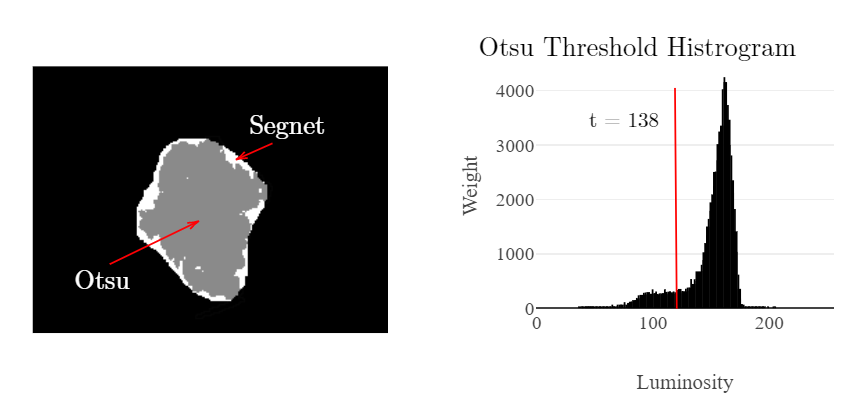
\includegraphics[scale=0.7]{otsu3.png}
\caption{Otsu thresholding alongside ground-truth mask, where grey Otsu and white is SegNet. The bar chart shows the histogram with an otsu threshold of 138.} \label{otsu2}
\end{figure}

\subsection{Results}
Both statistical models of LBPC and Otsu threshold generated accurate border cut-off as compared to the machine learning approach SegNet. Measuring border cut-off exaggerates irregular borders successfully, making it helpful in detecting border irregularities and possibly with other ABCD rules. It might be beneficial to combine SegNet and LBPC by using SegNet to find the skin lesions location, followed by adjusting the border cut-off using LBPC.

\section{Extracting ABCD Rules Feature Components}
This section describes extracting features from the ABCD rules in various ways for comparison. The ground-truth masks are being used in this section instead of the generated segmentation masks to measure the quality of results fairly.

\subsection{Centroid and Rotation using Spatial Moments}
Spatial moments locate the centroid of a skin lesion (using a segmentation mask) to measure shape asymmetry using bi-folds, using the right angle from the centroid to find the closest fit for both axes. For example, equation \ref{eq2} describes a two-dimensional spatial moment of $M_{ij}$ being generated from the pixel intensity $I$ and locations $x$ and $y$, generating an array of moments Where an array. Then, a set of algorithms calculate the centroid and rotation of the skin lesion.

\begin{equation} \label{eq2}
M_{ij}=\sum_x\sum_yx^iy^jI(x,y)
\end{equation}

Equation \ref{eq3} demonstrates the centroid $C$ calculated using the array of moments. The equation uses the ground-truth (mask) to calculate the centroid, whereas grayscaled images find a different centre depending on the weight distribution.

\begin{equation} \label{eq3}
C_x = \frac{M_{10}}{M_{00}}\qquad
C_y = \frac{M_{01}}{M_{00}}
\end{equation}

The algorithm described in \ref{eq4} uses the calculated array of moments $M$ to estimate the rotation. However, rotation is only related to shape, not colour or texture. For example, comparing asymmetry colour and texture always relies on the moment rotation calculated using the shape without consideration for colour or texture. Therefore, modifying the moments' rotation to consider colour and texture might improve measuring colour and texture accuracy.

\begin{equation} \label{eq4}
i(\phi) = 0.5\tan^{-1}[\frac{2M_{11}}{M_{20}-M_{02}}]
\end{equation}

\subsection{Bi-fold Asymmetry Measurements}
Bi-folds are a statistical technique for measuring the asymmetry of skin lesions. Described in this section are two techniques for measuring shape and colour.

\subsubsection{Shape}
Bi-fold shape measures the asymmetry of skin lesions as described in the ABCD rules. Diagram \ref{asy1} demonstrates shape bi-folds of an atypical and typical skin lesion by splitting the skin lesion four halves down the centroid (found using moments) and folding each perpendicular line horizontally and vertically to subtract the halves. Each vertical and horizontal pixel is summed and compared to a threshold, assigning a 0, 1 or 2. The value 0 is a near-perfect overlap on both axes making it typical; 1 is a horizontal or a vertical overlap is atypical, and 2 is both horizontal and vertical overlaps are atypical.

\begin{figure}
\centering
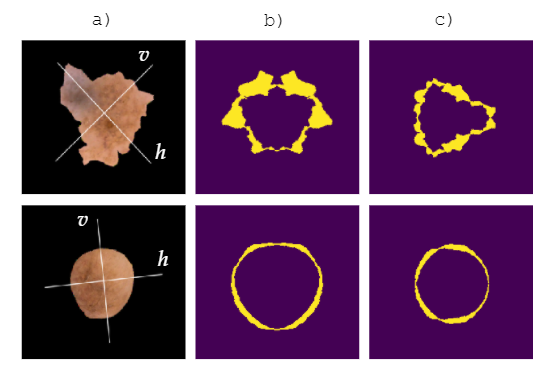
\includegraphics[scale=1.2]{shape.png}
\caption{Using a bi-fold to find whether the shape of the skin lesion is asymmetrical, a) two skin lesions (in order) with of asymmetrical (TDS = 2) and symmetrical (TDS = 0), b) vertical bi-folds, and c) horizontal bi-folds}
\end{figure} \label{asy1}

The equation \ref{shape} calculates the difference between symmetrical sides, where $p_0$ is the vertical comparison, $p_1$ is the horizontal comparison, $g$ is the total number of pixels of the original mask, $h$ is the total amount of pixels from horizontal, and $v$ is the total amount of vertically un-subtracted pixels.

\begin{equation} \label{shape}
p_0 = \frac{h-g}{h}\qquad
p_1 = \frac{v-g}{v}
\end{equation}

Equation \ref{shape2} and \ref{shape3} demonstrates generating the TDS of 0, 1, or 2 for measuring asymmetry. A vertical and horizontal comparison of $p_i$ where $i=2$ is compared to a threshold $t$, producing a value between 0 and 1. The addition of the calculated values $s_0$ and $s_1$. This score is beneficial to doctors because its output follows TDS, and the algorithm itself is simple and easy to understand. However, the accuracy of 58.5\% using the PH$^2$ dataset with a threshold of 108 demonstrates a need for further advancement.

\begin{equation} \label{shape2}
s_i
\begin{cases}
1,\:\:p_i\geq\:t; \\
0,\:$otherwise$.
\end{cases}
\end{equation}

\begin{equation} \label{shape3}
TDS = s_0 + s_1
\end{equation}

\subsubsection{Colour}
Measuring the colour distribution involves splitting the skin lesion into 10x10 averaged squares of colour as described in figure \ref{asy-graph1}. Then, the bi-fold and moments measure the centroid by splitting the skin lesion horizontally and vertically, comparing each perpendicular colour using the 3-dimensional euclidean distance.

\begin{figure}
\centering
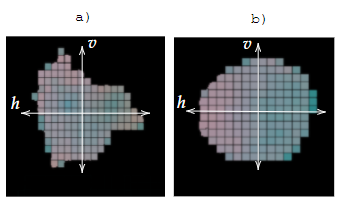
\includegraphics[scale=1.2]{asym-colour.png}
\caption{Splitting the skin lesion into a grid and averaging each square to measure the asymmetry of colour. Each square is compared with the opposite square the same distance away from each line.} \label{asy-graph1}
\end{figure} 

The graphs in figure \ref{asy-graph2} show each colour comparison of either side of the vertical and horizontal axes. The skin lesion used to measure this is the atypical one mentioned in \ref{asy1}. More than half the points are higher than the threshold of 10; therefore, the vertical is considered asymmetrical in colour. According to the PH$^2$ dataset, this image is symmetrical, but the colour difference describes otherwise. The described skin lesion has a specular reflection fading from one side to another. The lesion is then considered symmetrical by removing the v value from HSV.

\begin{figure} 
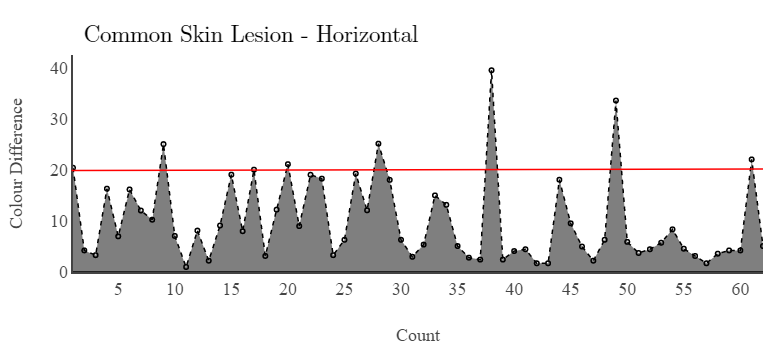
\includegraphics[scale=0.7]{common-h.png}
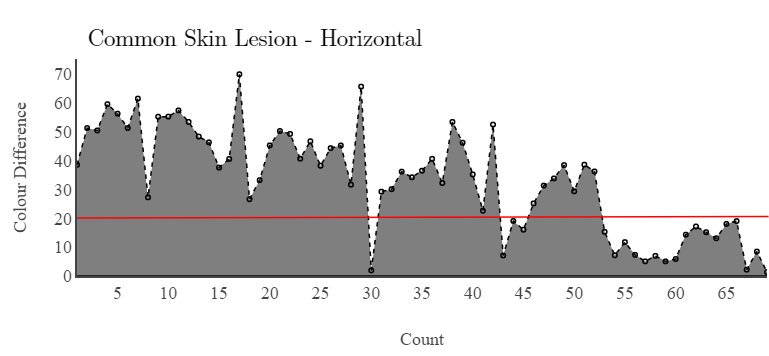
\includegraphics[scale=0.7]{common-v.png}
\caption{Bi-Fold colour asymmetry measurements using euclidean distance of the HSV, where each position represents the difference in colour from its perpendicular square.}\label{asy-graph2}
\end{figure} 

In equations \ref{hor} and \ref{ver} calculate the colour asymmetry. Horizontal as $h$ and vertical as $v$ are the combined sum of the subtracted sides where $p$ each bi-fold (four in total), $(x,y)$. Furthermore, because the data is a one-dimensional array, but the data is considered two-dimensional, size as $s$ is used to navigate, equal to 10. Comparing the results to a threshold of 20, where more than half are above the threshold, adds an asymmetrical score of 1. The 0, 1 or 2 scores followed the same criteria for measuring the border as TDS used in clinical environments, which is beneficial to doctors because it is interpretable. The accuracy is 59.5\% with a threshold of 20 using the PH$^2$ dataset.

\begin{equation} \label{hor}
h = p_0(x*s+y) - p_1(s^2-(x*s)+y)
\end{equation}

\begin{equation} \label{ver}
v = p_2(x*s+y) - p_3(x*s+(s-y))
\end{equation}

\subsection{Box-Counting Fractal Dimensions}
Box-counting, otherwise known as the Minkowski dimension, is a type of fractal geometry for measuring the complexity of an image. This algorithm aims to classify complex structures from smooth structures by maximising a score of $R$ based on the input data. For example, smoother structures will have a lower score than complex structures with a higher score. In contrast, typical melanoma sometimes has an irregular border with ridges, corners, and ledges \cite{Kaya2016}, compared to benign lesions that are essentially an oval shape. Therefore, melanoma is likely to have a higher overall score, making it a promising method for classification.

Figure \ref{boxcounting} has an irregular border (which is an oval) of a skin lesion that, using the contour positions of the border between the distance and the centre, was flattened. Next, a grid is applied of factor $S$ counting each box overlapping with the line, making the value $N$. Finally, table \ref{boxcounting2} shows the individual log of $S$ and $N$, creating the values that will be utilised in a line graph to calculate the fractal $R$ = 0.996.

\begin{figure}
\includegraphics[scale=0.9]{box-counting.png}
\caption{Box-counting where number of boxes is N and the factor (S) is the size of the grid scaling from 0, 2, 4, and 8.}\label{boxcounting}
\end{figure} 

\begin{table}
\begin{tabular}{ c|c c c c }
 Factor (S) & 0 & 2 & 4 & 8 \\
 log(S) & 0 & 0.3010299957 & 0.6020599913 & 0.903089987 \\
 \hline  
 Number of Boxes (N) & 16 & 37 & 75 & 141 \\
 log(N) & 1.204119983 & 1.568201724 & 1.875061263 & 2.149219113  
\end{tabular}
\caption{Log(S) is calculated from the values of factor(S) and log(N) is calculated from the number of boxes (N).} \label{boxcounting2}
\end{table}

A line graph with $log(S)$ as X and $log(N)$ as Y with a base of 10 calculates the fractal $R$. Next, a trendline generates the fractal score of 0.996, as shown in figure \ref{boxcounting3}. Typically, this value ranges from 0 and 2, where 0 is simple, and 2 is complex. This value is stored as a single vector and combined with Zernike moments and convexity to measure border irregularity \cite{Ali2020b}.

\begin{figure}
\centering
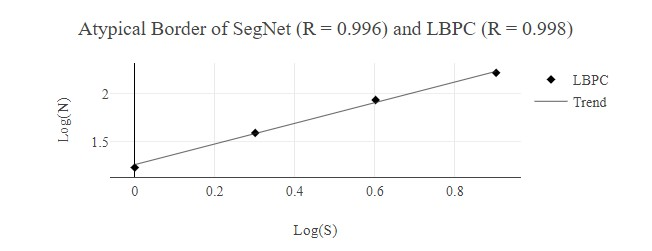
\includegraphics[scale=0.9]{box-counting2.jpg}
\caption{Line graph of values log(S) and log(N) making a fractal score R = 0.996.}\label{boxcounting3}
\end{figure}

\subsection{Results}
Statistical techniques including bi-fold and box-counting are substantial for extracting asymmetry and border interpretably regarding the ABCD rules. However, the asymmetry shape has 58.5\% and colour accuracy of 59.5\%, which is substantially low. A group of statistical features train an SVM model, similar to measuring border irregularity with box-counting, convexity, and Zernike moments \cite{Ali2020b} to improve the accuracy. Therefore, utilising a group of extracted features together, such as asymmetry shape, colour, and texture, might improve the accuracy.

\section{Experimental}

\subsection{Comparison of Border Irregularity Detection by Adjusting Border Cut-off Using SegNet and LBPC}

Many papers \cite{Ali2020b} discuss that generating an accurate border cut-off between skin and skin lesions improves the classification accuracy of measuring border irregularity. To demonstrate this, two skin lesions, one with an irregular border and another with a regular border, are both segmented using SegNet and LBPC. Next, comparing each of the four using fractal box-counting to reach a fractal score of $R$, where an increased score (between 0 and 2) demonstrates an irregular border with ledges and corners. In comparison, a lower score demonstrates a regular border that is smooth and oval. This validation uses two images from the PH$^2$ dataset as a brief comparison and will be tested on a larger scale later.

Figure \ref{fractal2} demonstrates the fractal box-counting method where the number of boxes  $N$ that overlap and the increment of the grid size are $S$. Values of $S$ has a higher score of 1 for LBPC than SegNet because of the increased ridge depth of the images. Furthermore, figure \ref{fractal3} demonstrates the regular border that has an increased box-count of $N$ between SegNet and LBPC. Factor (S) increases from 0, 2, 4, and 8, where four values as needed to calculate the fractal dimension $R$.

\begin{figure}

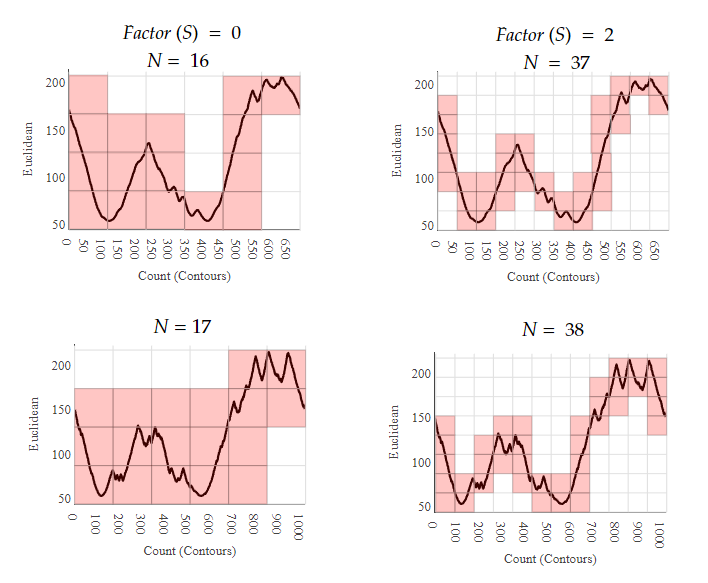
\includegraphics[scale=0.9]{lbpcvseg.png}

\caption{Comparison of an irregular skin lesion border between SegNet and LBPC using fractal box-counting where size is $S$ and number of boxes is $N$.} \label{fractal2}
\end{figure}
\begin{figure}
\centering

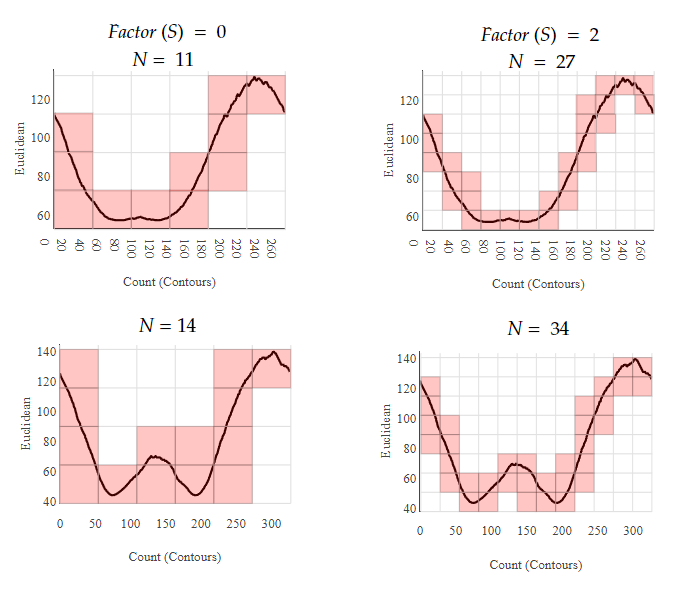
\includegraphics[scale=0.9]{lbpcvseg2.png}

\caption{Comparison of a regular skin lesion border between SegNet and LBPC using fractal box-counting where size is $S$ and number of boxes is $N$.} \label{fractal3}
\end{figure}

Figure \ref{fractal4} shows the difference between SegNet and LBPC, where SegNet has the lower box-count ($N$) each time. Interestingly the regular border decreases in value as the size $S$ increases, and the fractal score ($R$) decreases from 0.99 to 0.85 when using LBPC. In comparison, the irregular border fractal score increases from 0.996 to 0.998. Overall, utilising LBPC exaggerates an irregular border successfully whilst lessening the regular border. Therefore, the border cut-off can improve the classification accuracy for border analysis techniques regardless of these segmentations not matching that of datasets annotated by dermatologists. 

\begin{figure}
\centering
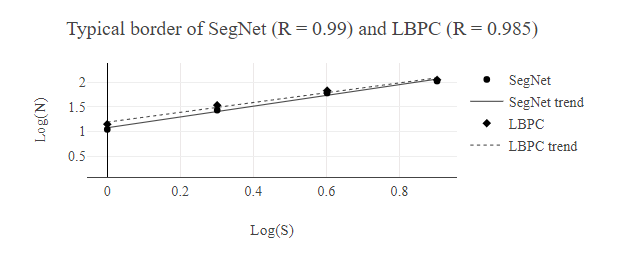
\includegraphics[scale=0.9]{typicalborder.png}
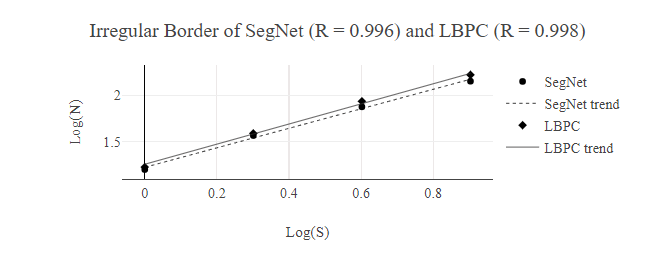
\includegraphics[scale=0.9]{atypicalborder.png}

\caption{Comparison of SegNet and LBPC with regular and irregular border types. LBPC successfully exaggerates irregular borders from 0.996 to 0.998 while simultaneously decreasing the value of a regular border from 0.99 to 0.985.} \label{fractal4}
\end{figure}

\subsection{Improved Asymmetry Classification of Colour Distribution Using Superpixels}
The goal of this experiment is to improve the accuracy of the asymmetry bi-fold technique described by Ihab S. Zaqout et al. \cite{Zaqout2016}. Initially, the skin lesion is split into a 10x10 grid and converted into the LAB colourspace. Next, a line is drawn through the middle horizontally and vertically. Measuring the euclidean distance from the centroid, locating the closest opposite patch of colour finds the parallel square. Subtracting the squares generates a score for each value, the closer to 0, the more similar the colour. These are then removed from the list to prevent them from being selected a second time. If half the results are over a specific threshold, it is considered asymmetrical in colour, otherwise considered symmetrical. The aim is to make a 10x10 grid, but instead of averaging squares, superpixels reduce data redundancy in the grid, allowing for a less complex algorithm and improving accuracy. The clustering method k-means partition each pixel to its nearest most similar centroid relating to colour. Next, it generates a superpixel that represents the average colour of that area. The diagram \ref{SP} demonstrates different borders when changing the $C$ for compactness, where 100 generates a square grid similar to the original technique. The border becomes more flexible as the compactness value decreases.

\begin{figure} 
\centering
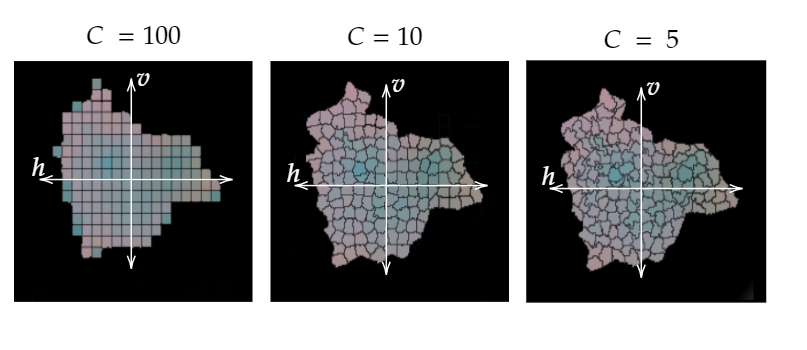
\includegraphics[scale=0.6]{superpixels.png}
\caption{This diagram shows the skin lesion split relating to superpixels instead of averaging squares.}
\end{figure} \label{SP}

Each parallel square on the vertical and horizontal axes measures similarity using a three-dimensional euclidean distance in the LAB colourspace. For example, the perceivable difference of colour to the human eye is a three-dimensional euclidean distance of 6 \cite{Myridis2014a}. Using similar logic, a value of 20 is the threshold, where any value over that amount is considered asymmetrical in colour. Next, each square is compared with its closest parallel square and removed from an array after being compared. The next improvement is to generate a unique threshold for the significance of each square. For example, using superpixels with the compactness of 10 has an accuracy of 61\% with the PH$^2$ dataset compared to the original 59.5\%. This approach demonstrates that a flexible border that considers features is more effective than averaging squares.

\begin{figure}
\centering
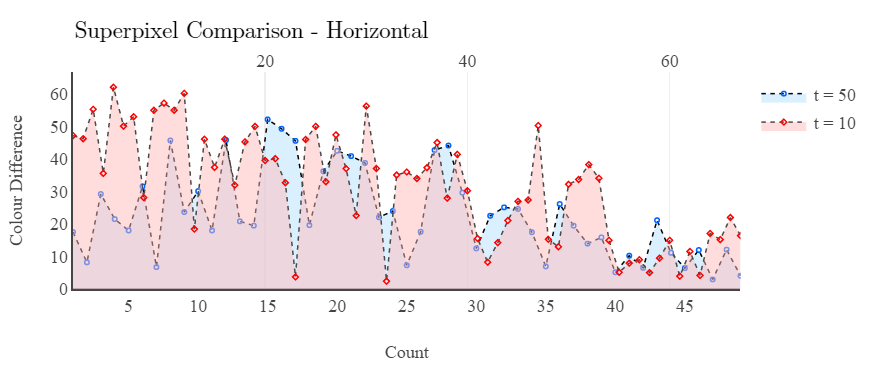
\includegraphics[scale=0.7]{superpixel2.png}
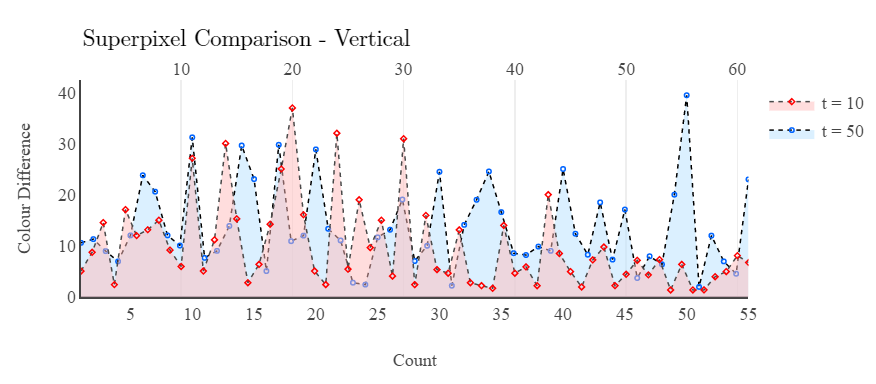
\includegraphics[scale=0.7]{superpixel1.png}
\caption{This diagram shows the difference between averaging squares and using superpixels, with the threshold of 10 implying curves and 50 being square. The horizontal colour difference is improved, making it more likely to be seen asymmetrical. The vertical comparison is roughly the same, except for removing a false positive of 40.}
\end{figure} \label{asy3}

There is a correlation in colour differences between the inner and outer edges because melanoma typically expands outwards, creating an abnormal border. This information specifies that the statistical model accuracy could be improved by increasing the threshold for the outer edges and decreasing for the inner.

\chapter{Conclusion}
Validating the automatic ABCD rules is challenging because public datasets are scarce and often lack sufficient data. For example, PH$^2$ contains 200 images on asymmetry, colour, and some dermoscopic structures but misses border irregularity. Therefore researchers aiming to measure borders use private or privately annotated datasets. Furthermore, many papers measuring asymmetry, colour and dermoscopic structures lack validation using public datasets despite PH$^2$ being available at the date of their publication. On the other hand, public datasets are crucial to comparing, validating, and reproducing algorithms. Therefore ABCD rules (apart from the border) will be validated using PH$^2$ datasets so that future researchers can replicate techniques. Furthermore, once rules are combined using Bayesian fusion, a type of probabilistic analysis, results can conform to the diagnosis between malignant and benign, validated from larger datasets, including ISIC 2019.

Finding the border cut-off is fundamental for the classification of melanoma using the ABCD rules \cite{Pereira2020}. Many valuable techniques use statistical models, including LBPC and Otsu, instead of transposed CNNs such as SegNet. Hybrid approaches using SegNet followed by Otsu to measure the border cut-off have been proven beneficial. However, using SegNet without a statistical model is worse when used with the ABCD rules than current methods such as LBPC and Otsu. Therefore, exploring other statistical segmentation techniques and hybrids would be beneficial. Furthermore, segmentation ground-truths do not always correspond to good classification accuracy with ABCD rules, which means even a low accuracy segmentation compared to datasets might have better accuracy when classifying the ABCD rules for border irregularity.

Statistical models for asymmetry, border, and colour extract relevant features for melanoma classification. The goal is to mimic the diagnostic procedure that clinicians are familiar with to produce results that they can utilise in a clinical environment. Extracting relevant features using box-counting and bi-folds ensures capturing relevant features and that the technique is retractable. However, accuracy is lacking in these techniques where superpixels improved asymmetry, changing the accuracy from 58.5\% to 61\% for the PH$^2$ dataset. Further improvements will be made after training an SVM model using the extracted features. Further implementation of convexity and Zernike moments for border irregularity will improve the accuracy. Furthermore, implementing a texture comparison for asymmetry measurements improve accuracy again.

\chapter{Future Work}
Developing algorithms to extract features of ABCD rules is beneficial to GPs because it improves interpretability. Future work will involve extracting more features and training SVM models. For example, extracting more relevant asymmetry features will help classify asymmetry as there is currently no unification of shape, colour, and texture into a single classification model. The extracted features will be combined into a diagnosis between benign and malignant using a Bayesian probabilistic network. Bayesian probability is beneficial because its highly accurate \cite{Takruri2017} and modifiable and ability to classify with incomplete data. For example, asymmetry, border, and colour are sometimes enough to classify skin lesions. However, in some cases, dermoscopic structures or other meta-data, including age, gender, touch, feeling, and location on the body, are required for an accurate diagnosis. Furthermore, This might benefit GPs because it encourages considering a wide range of not always considered features.

Melanoma evolves from benign lesions at initially 30\%-50\%, and despite its significance, clinicians or computers are not yet able to reliably predict this change. AI trained on relevant images could predict melanoma before it occurs \cite{Sondermann2019}. Data on skin lesion evolution is rare in public datasets. However, the associated organisation has taken images of the same skin lesion multiple times. It would be incredibly beneficial to assess the quality of these images, which could potentially lead to the development of a technique describing evolution. Considering evolution in machine learning techniques in the future would be incredibly beneficial to the early detection of melanoma but can only be achieved when there is more data.


\global\pdfpageattr\expandafter{\the\pdfpageattr/Rotate 90}
\section{Project Schedule}
\centering
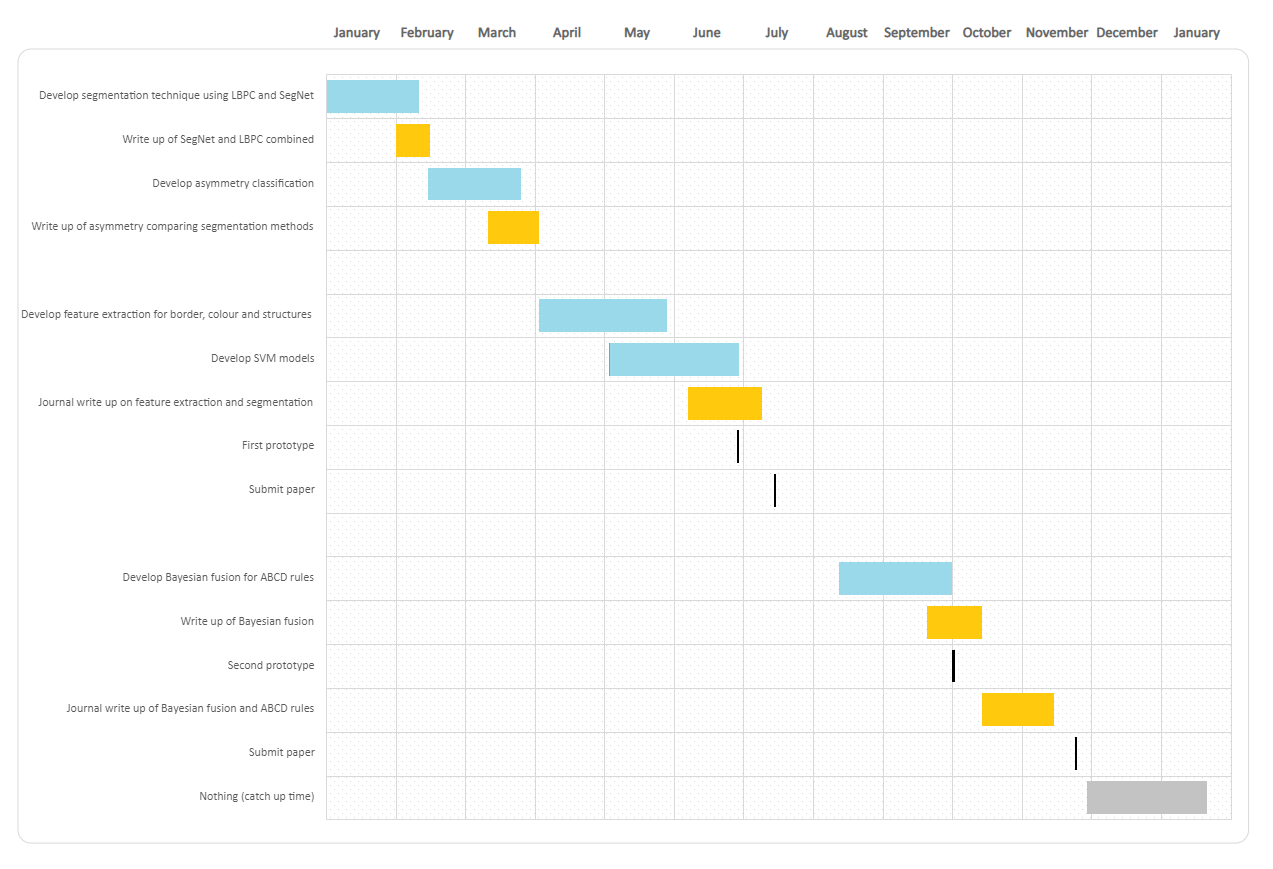
\includegraphics[angle=90, scale=0.6]{gantt.PNG}
\pagebreak[4]
\global\pdfpageattr\expandafter{\the\pdfpageattr/Rotate 0}
\bibliographystyle{unsrt}
\bibliography{PHD-ElliotNaylor}

\end{document}



